\subsection{Dispositivo}

El prototipo, al conectarse a una red eléctrica iniciará el asistente, al igual que dejará corriendo en segundo plano el subproyecto que hemos desarrollado con el fin de poder controlar y monitorizar el propio dispositivo.

\subsubsection{Naturaleza del controlador}

El monitoreo y control remoto de un dispositivo plantea el siguiente dilema: cómo invertir los roles para que un cliente haga de servidor recibiendo información, mientras el servidor hace de cliente mandando a este peticiones.

Para resolver esta adversidad se toma una visión general del proyecto:
\begin{enumerate}
    \item El dispositivo informa cada cierto tiempo de que sigue encendido.
    \item El servidor proporciona una API REST.
\end{enumerate}

Como bien se sabe, los operaciones básicas de una API REST son \textit{GET, POST, PUT y DELETE}, de modo que si se hace una petición \textit{GET} para informar sobre su conexión activa a la red eléctrica, se puede aprovechar por parte del servidor esta llamada para inyectar una acción a realizar en el dispositivo como respuesta a esta llamada.

De este modo el servidor podría manejar el dispositivo, monitorizándolo o pidiendo que haga acciones de manera remota, pudiendo tratarse por ejemplo de una tarea cuya finalidad sea que el asistente inicie una conversación con el usuario final en caso de que haya habido un accidente, de manera que se le pueda ayudar.

Este planteamiento en cuanto a la naturaleza del controlador y su modo de uso parece factible, pero tiene la pega de la usabilidad, ya que si el dispositivo tiene una configuración de mandar su estado cada 24 horas, el control del dispositivo se demoraría demasiado, y aquí entra en juego la siguiente técnica:

Se puede configurar en el propio dispositivo que las 24 horas que pasa entre aviso y aviso se obtengan a partir de un fichero de configuración, que permita la variación de estas 24 horas.
También, en segundo plano, se puede configurar que a ciertas horas, el dispositivo disminuya su periodo de aviso, coincidiendo con unas ciertas horas relativas al horario del admnistrador del sistema, de modo que este pueda mandarle una primera tarea que sea otra reducción del periodo de aviso, por ejemplo a 10 segundos, permitiendo una comunicación síncrona más pareja a una comunicación real, y permitiendo un envío posterior de tareas al dispositivo que se realizarían en un espectro corto de tiempo.

En la figura \ref{fig:prototype-flow} se puede observar el flujo de estados propuesto e implementado en este proyecto con el fin de poder controlar y monitorizar el dispositivo.

\begin{figure}[h!]
    \centering
    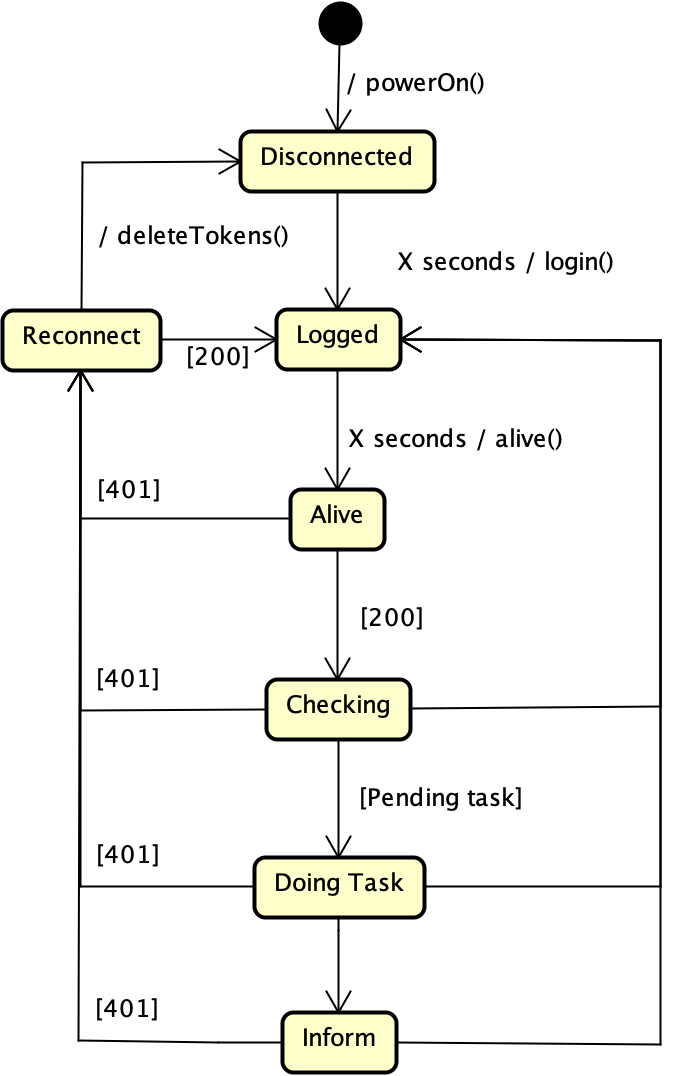
\includegraphics[width=7cm]{./img/state/prototype-flow.png}
    \caption{Flujo de estados del dispositivo}
    \label{fig:prototype-flow}
\end{figure}

\subsubsection{Desarrollo}
Una vez planteada al teoría de cómo debe funcionar el asistente, toca ponerse con la práctica y demostrar que se puede formar un sistema que funcione y sea escalable.

Para ello, se establece un espacio de trabajo dentro del dispositivo, el cual se vincula con un proyecto alojado en un servicio de control de versiones.
De esta manera, se permite la posibilidad de actualizar las acciones del dispositivo con tan solo realizar una acción \textit{pull} del repositorio de origen.

%% Sistema de arranque
\textit{\textbf{Sistema de arranque}}

El sistema implementado se ejecutará en el momento en el que se ejecute la clase \textit{Main.py}, que intenta iniciar sesión con el servidor a través del método \textit{signin()} de un objeto obtenido a través de la clase \textit{Login.py}.
En el momento de instanciación del objeto \textit{login}, su constructor obtiene la dirección MAC del dispositivo, almacenándola en: 
\begin{center}
\textit{./cache/macfile.txt}
\end{center}

Esta dirección MAC propia y única para cada dispositivo, será utilizada como identificador en los credenciales a la hora de identificarse contra el servidor.
La contraseña, será una encriptación de la dirección MAC que se obtiene simultáneamente en el constructor.

Si se consigue iniciar sesión, se almacenan los tokens tanto en el objeto instanciado, como en el siguiente fichero externo:
\begin{center}
\textit{./cache/tokens.json}
\end{center}

Este almacenamiento externo permite su utilización a futuros programas que requieran los tokens para realizar peticiones contra el servidor. Continuando con el método el cual inició sesión, este devuelve un booleano, \textit{true}, desbloqueando un semáforo del \textit{main} que permite el envío al servidor del estado actual del dispositivo, a través de un método perteneciene a un objeto de tipo \textit{Alive.py}, el cual devuelve también otro booleano, que será \textit{false} en caso de que no se lleve la acción correctamente a cabo, cerrando el semáforo.

Tras la implementación de este flujo de estados se ha podido comprobar la perfecta sincronía con el servidor, permitiendo proceder al diseño de un sistema que acepte la implementación de tareas.

%% sistema de tareas
\textit{\textbf{Sistema de tareas}}

En el momento en el cual se hace la petición de \textit{/alive}, existen tres posibles respuestas por parte del servidor:
\begin{enumerate}
    \item \textit{HTTP Status Code 200}: indica que la petición ha sido correcta.
    \item \textit{HTTP Status Code 300}: indica que la petición ha sido correcta, pero que hay múltiples respuestas, indicando al sistema del dispositivo que debe extraer la información que contiene el mensaje. En este mensaje, se incluye una lista de tareas pendientes del dispositivo:
    
\begin{lstlisting}
[{
    "id" : "task identifier",
    "device" : "device identifier",
    "event" : "TAREA",
    "by" : "who ordered this",
    "at" : "when it was ordered"
}]
\end{lstlisting}


    \item \textit{HTTP Status Code 401}: indica que el token ha dejado de ser válido, por lo que se debería volver a iniciar sesión, o refrescar el token. Como un token de acceso tiene establecido por razones de seguridad un tiempo de validez de 30 minutos, y el dispositivo en principio realizará la petición de mostrar que sigue activo cada 24 horas, no se ve necesaria la implementación en el dispositivo de un método que refresque el token, ya que produciría un aumento del consumo de datos, al refrescar constantemente un token al que no va dar uso.
    
\end{enumerate}

Una vez recibida una respuesta de tipo \textit{HTTP Status Code 300}, se procede a analizar las tareas pendientes que están en el cuerpo del mensaje. Para ello, se procede a ejecutar siempre la primera de la lista gracias a que han sido devueltas por orden de asignación desde el servidor.
Analizando los campos de la tarea, vemos que dispone de campo llamado \textbf{event}, el cual indica el nombre de la tarea a realizar.

El nombre de la tarea es único, y debe ser una palabra sin espacios, permitiendo utilizarlo como palabra clave.
Gracias a esta palabra clave, se puede pedir al dispositivo que ejecute la tarea concreta, y para ello administramos el sistema de ficheros de modo que siga la siguiente estructura:

\begin{center}
    \textit{/task/TAREA/}
\end{center}
y dentro de ese directorio, debe haber un script, el cual ejecute la tarea específica:

\begin{center}
    \textit{/task/TAREA/init.sh}
\end{center}

\begin{figure}[h!]
    \centering
    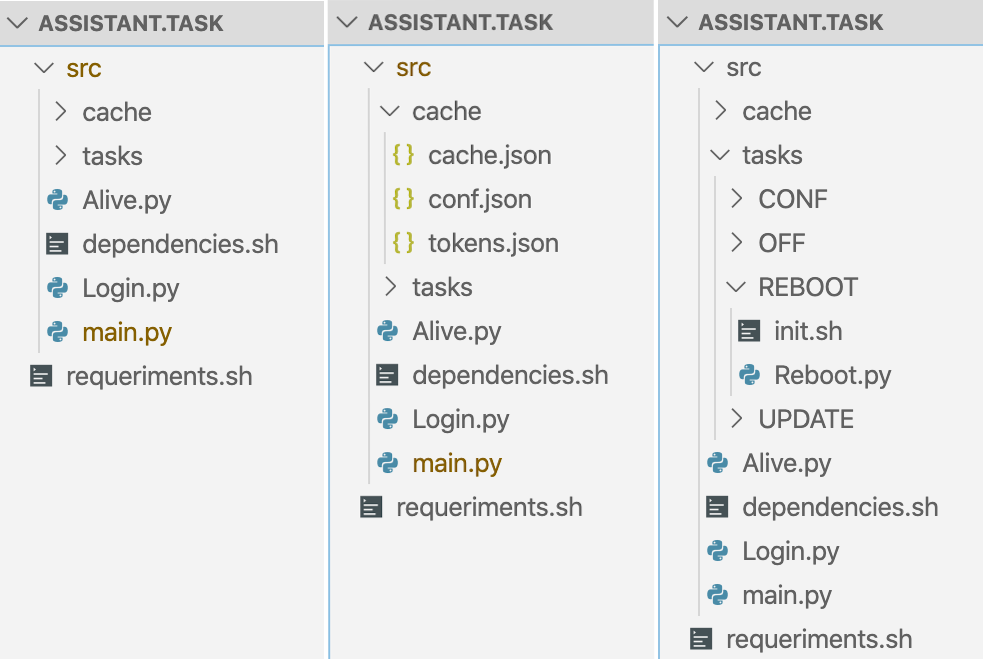
\includegraphics[width=10cm]{./img/arch/device/src.task.png}
    \caption{Contenido global del repositorio}
    \label{fig:src.task}
\end{figure}

Este script, puede llamar a otros programas o a otros scripts, de modo que se permite la realización de cualquier evento configurado.

Una vez se tiene esta estructura implementada, como se puede observar en la figura \ref{fig:src.task}, tan solo hay configurar que al recibir como respuesta del servidor un código 300, se ejecute el script que está almacenado en la dirección obtenida al sustituir el nombre de la tarea, por ejemplo, \textbf{REBOOT}, en la ruta base:

\begin{lstlisting}
    sh ./task/REBOOT/init.sh
\end{lstlisting}

Como se puede observar, este método de organización de tareas posibilita la fácil implementación de nuevas tareas sin poner en peligro las ya creadas, ya que únicamente se necesita crear un directorio nuevo por cada nueva tarea, y un script que inicie las acciones a realizar.

%% estructura global



%% inicio automático
\textit{\textbf{Inicio automático}}

Ya se tiene una configuración válida para el dispositivo, pero hay que poder asegurar su buen despliegue e inicio al reiniciar el dispositivo, de modo que se pueda tener como un valor seguro que, si un usuario reinicia la máquina físicamente, este dispositivo será capaz de iniciar el sistema ahora creado para poder monitorizarlo y controlarlo.

Entonces, para la configuración del espacio de trabajo se proporciona un script que permite la configuración del dispositivo en caso de ser la primera vez que se utiliza ese dispositivo, por si no se han cargado bien los servicios.

En dicho script, almacenado como \textit{requirements.sh}, se establecen dos pasos claves del proyecto:

\begin{enumerate}
    \item La configuración para el inicio automático del sistema de control remoto del dispositivo a través de la herramienta de \textit{crontab} que proporcionan los sistemas Unix.
    
\begin{lstlisting}
# configure scheduled task
(crontab -l ; echo "@reboot sleep 60; cd /home/pi/assistant.task/src/ ; python /home/pi/assistant.task/src/assistant-alive.py & > home/pi/assistant.task/src/cache/logfile.txt") | crontab -
\end{lstlisting}

De este modo, se abre el fichero de configuración de \textit{crontab} en el cual se plasma qué es lo que se desea que se ejecute en cada reinicio, como indica la etiqueta \textit{@reboot}.
Si se presta atención al script, se solicita una espera de 60 segundos a partir del reinicio del dispositivo, y el motivo por el cual se establece ese tiempo es para permitir que el dispositivo pueda configurar su conexión a internet y levantar previamente todos sus servicios antes de que el sistema aquí descrito arranque, evitando posibles interferencias que no permitiese arrancar de la manera correcta, como puede ser una mala obtención de la dirección MAC de la tarjeta de red.

\item El script de lo requisitos ejecuta otro script, el de la instalación de las dependencias, el cual permite la instalación de las librerías de python requeridas para el correcto funcionamiento del dispositivo.

\begin{lstlisting}
# install python dependencies
sudo sh ./src/dependencies.sh
\end{lstlisting}

\end{enumerate}


\begin{figure}[h!]
    \centering
    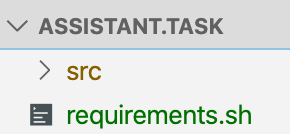
\includegraphics[width=3cm]{./img/arch/device/src.web.global.png}
    \caption{Contenido global del repositorio}
    \label{fig:src.web.global}
\end{figure}

\subsection{BackEnd}


    \subsubsection{Patrones}
    
    \subsubsection{servicios}
    
    \subsubsection{diagrama de clases}
    
    \subsubsection{diagrama entidad relacion}

    \subsubsection{End-Points}
    
\subsection{FrontEnd}

    \subsubsection{Estructura de directorios}
    
    \subsubsection{ (Pre)diseño de interfaz }
    
    \subsubsection{ Lógica }